\begin{frame}{Motivation}
\begin{block}{Apprentissage global ou ``ciblé''}
\begin{itemize}
 \item Le plan d'expérience a une influence très forte sur la précision locale
 \item Une bonne précision n'est pas nécessaire partout !
\end{itemize}
\end{block}

\begin{figure}
\centering
\includegraphics[width=\textwidth]{figT/two7pointskrigs.png} 
\end{figure}

\begin{alertblock}{Dans cette section}
 Un \textit{exemple} de plan séquentiel adapté à l'objectif
\end{alertblock}
\end{frame}

%%%%%%%%%%%%%%%%%%%%%%%%%%%%%%%%%%%%%%%%%%%%%%%%%%%%%%%%%%%%%%%%%%%%%%%%%%%%%%%%%%%%%%%%%%%%%%%%
\begin{frame}{Propagation d'incertitudes et analyse de risque (1/2)}
\begin{block}{Un problème classique : dépassement de seuil}
\begin{itemize}
 \item La sortie du simulateur doit rester sous une valeur critique (contraintes mécaniques, température, etc.)
 \item On connaît la loi des paramètres d'entrée
 \item On veut estimer : $\mathbb{P}\left[ y(X)\right] \geq seuil$
\end{itemize}
\end{block}

\vspace{10mm}
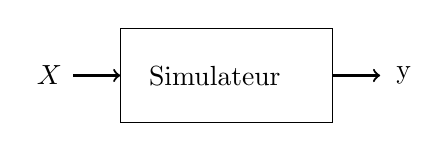
\begin{tikzpicture}[scale=0.3]
  \draw(0,1) node{$X$ };
   \draw[->,thick] (1,1)--(3,1);
  \draw(3,-1) rectangle (12,3);
  \draw(7,1) node{Simulateur};
 \draw[->,thick] (12,1)--(14,1);
 \draw(15,1) node{y};
 \end{tikzpicture}

\end{frame}
%%%%%%%%%%%%%%%%%%%%%%%%%%%%%%%%%%%%%%%%%%%%%%%%%%%%%%%%%%%%%%%%%%%%%%%%%%%%%%%%%%%%%%%%%%%%%%%%
\begin{frame}{Propagation d'incertitudes et analyse de risque (2/2)}
\begin{itemize}
 \item Approche par Monte-Carlo : on génère $X_1, \ldots, X_N$ $\Rightarrow$ $y(X_1), \ldots, y(X_N)$ et on compte 
 $$\frac{1}{N}\sum_{i=1}^N \mathbbmss{1}(y(X_i)) > T$$
\begin{figure}
\centering
\includegraphics[trim=0 0 200mm 0, width=.55\textwidth, clip]{figT/branin.png} 
\includegraphics[width=.4\textwidth]{figT/MCex.pdf} 
\end{figure}
 \item $y$ coûteux $\Rightarrow$ métamodèle
\end{itemize}
\end{frame}
%%%%%%%%%%%%%%%%%%%%%%%%%%%%%%%%%%%%%%%%%%%%%%%%%%%%%%%%%%%%%%%%%%%%%%%%%%%%%%%%%%%%%%%%%%%%%%%%
\begin{frame}{Problème considéré et métamodèle}

\begin{block}{Recherche de lignes de niveau}
\begin{itemize}
 \item On veut savoir si $y(\mathbf{x}) \geq T$
  \item $y(\mathbf{x}) \ll T$ or $y(\mathbf{x}) \gg T$: un métamodèle imprécis suffit
 \item Région critique pour l'apprentissage : $X_T = \left\{ \mathbf{x} / y(\mathbf{x}) \approx T \right\}$
\end{itemize}
\end{block}

On va enrichir le modèle pour qu'il soit précis dans la région critique.
\end{frame}

%%%%%%%%%%%%%%%%%%%%%%%%%%%%%%%%%%%%%%%%%%%%%%%%%%%%%%%%%%%%%%%%%%%%%%%%%%%%%%%%%%%%%%%%%%%%%%%%
\begin{frame}{Un exemple de critère pour l'apprentissage ciblé}
\begin{block}{Exploitation de l'information du modèle}
\begin{itemize}
	\item Région critique : $X_T = \left\{ \mathbf{x} / \left| y(\mathbf{x}) - T  \right| \leq \varepsilon \right\}$
	\item On peut calculer la probabilité $P\left(\mathbf{x} \in X_T \right)$:
	$$P\left(\mathbf{x} \in X_T \right) = \Phi \left( \frac{T + \varepsilon - m(\mathbf{x})}{s(\mathbf{x})} \right) - \Phi \left( \frac{T - \varepsilon - m(\mathbf{x})}{s(\mathbf{x})} \right)$$
\end{itemize}
\end{block}

\begin{block}{Critère IMSE ``ciblé''}
Variance de prédiction pondérée par la prédiction d'appartenir à la région cible :
$$IMSE_T = \int_D MSE(\mathbf{x}) P\left(\mathbf{x} \in X_T \right)d\mathbf{x}$$
\end{block}
\end{frame}
%%%%%%%%%%%%%%%%%%%%%%%%%%%%%%%%%%%%%%%%%%%%%%%%%%%%%%%%%%%%%%%%%%%%%%%%%%%%%%%%%%%%%%%%%%%%%%%%
\frame
{
\frametitle{Illustration: modification du critère IMSE}
$\mathbf{x}_{n+1} = \arg \min IMSE_T(\mathbf{x}_{new})$

\begin{figure}
  \centering
  \includegraphics[width=60mm]{figT/illustIMSETseq.png}
\end{figure}
}
%%%%%%%%%%%%%%%%%%%%%%%%%%%%%%%%%%%%%%%%%%%%%%%%%%%%%%%%%%%%%%%%%%%%%%%%%%%%%%%%%%%%%%%%%%%%%%%%
\frame
{
\frametitle{Illustration: 2 points initiaux + 7 itérations}
\begin{figure}
  \centering
  \includegraphics[width=85mm]{figT/illustOptIMSET.png}
\end{figure}

\scriptsize{
 \begin{thebibliography}{1}
\beamertemplatearticlebibitems
%\beamertemplatebookbibitems
     \bibitem{kriginv}
     C. Chevalier, V. Picheny, D. Ginsbourger
         \newblock KrigInv: An efficient and user-friendly implementation of batch-sequential inversion strategies based on kriging
         \newblock Computational Statistics and Data Analysis, 71, 1021-1034 (2014)
 \end{thebibliography}
}

}
%%%%%%%%%%%%%%%%%%%%%%%%%%%%%%%%%%%%%%%%%%%%%%%%%%%%%%%%%%%%%%%%%%%%%%%%%%%%%%%%%%%%%%%%%%%%%%%%
\begin{frame}{Exploitation pour un calcul de probabilité de défaillance}
\begin{block}{Problème jouet}
 \begin{itemize}
  \item Réponse dépendant de deux paramètres
  \item Entrées gaussiennes
  \item Seuil = 0
 \end{itemize}
\end{block}

\begin{figure} 
\centering
\includegraphics[width=\textwidth]{figT/branin.png} 
\end{figure}

\end{frame}
%%%%%%%%%%%%%%%%%%%%%%%%%%%%%%%%%%%%%%%%%%%%%%%%%%%%%%%%%%%%%%%%%%%%%%%%%%%%%%%%%%%%%%%%%%%%%%%%
\begin{frame}{Exploitation pour un calcul de probabilité de défaillance}

\begin{figure} 
\centering
\includegraphics[width=\textwidth]{figT/Pf.pdf} 
\end{figure}

Probabilité exacte : 1,75\% \\
Probabilité estimée : 1,69\%
\end{frame}
